\section{Answers to questions}

\subsection{Question 1}
\textit{Run the two algorithms you have implemented on the graphs of the dataset. For the Karger and Stein algorithm, use a number of repetitions that guarantees a probability to obtain a global min-cut of at least 1 - \(\frac{1}{n}\) .\\
Measure the execution times of the algorithms and create a graph showing the increase of execution times as the number of vertices in the graph increases. Compare the measured times with the asymptotic complexity of the algorithms. For each problem instance, report the weight of the minimum cut obtained by your code.\\
You can use a timeout to limit the execution time of large instances if it became too large.
}\\ \\
\noindent
We have implemented the code in C\# for the execution of the \textbf{Stoer-Wagner}'s algorithm on the whole provided dataset.
The results are reported in detail with the relative weights also in the appendix section (\ref{stoer}).

\begin{figure}[H]
	\centering
	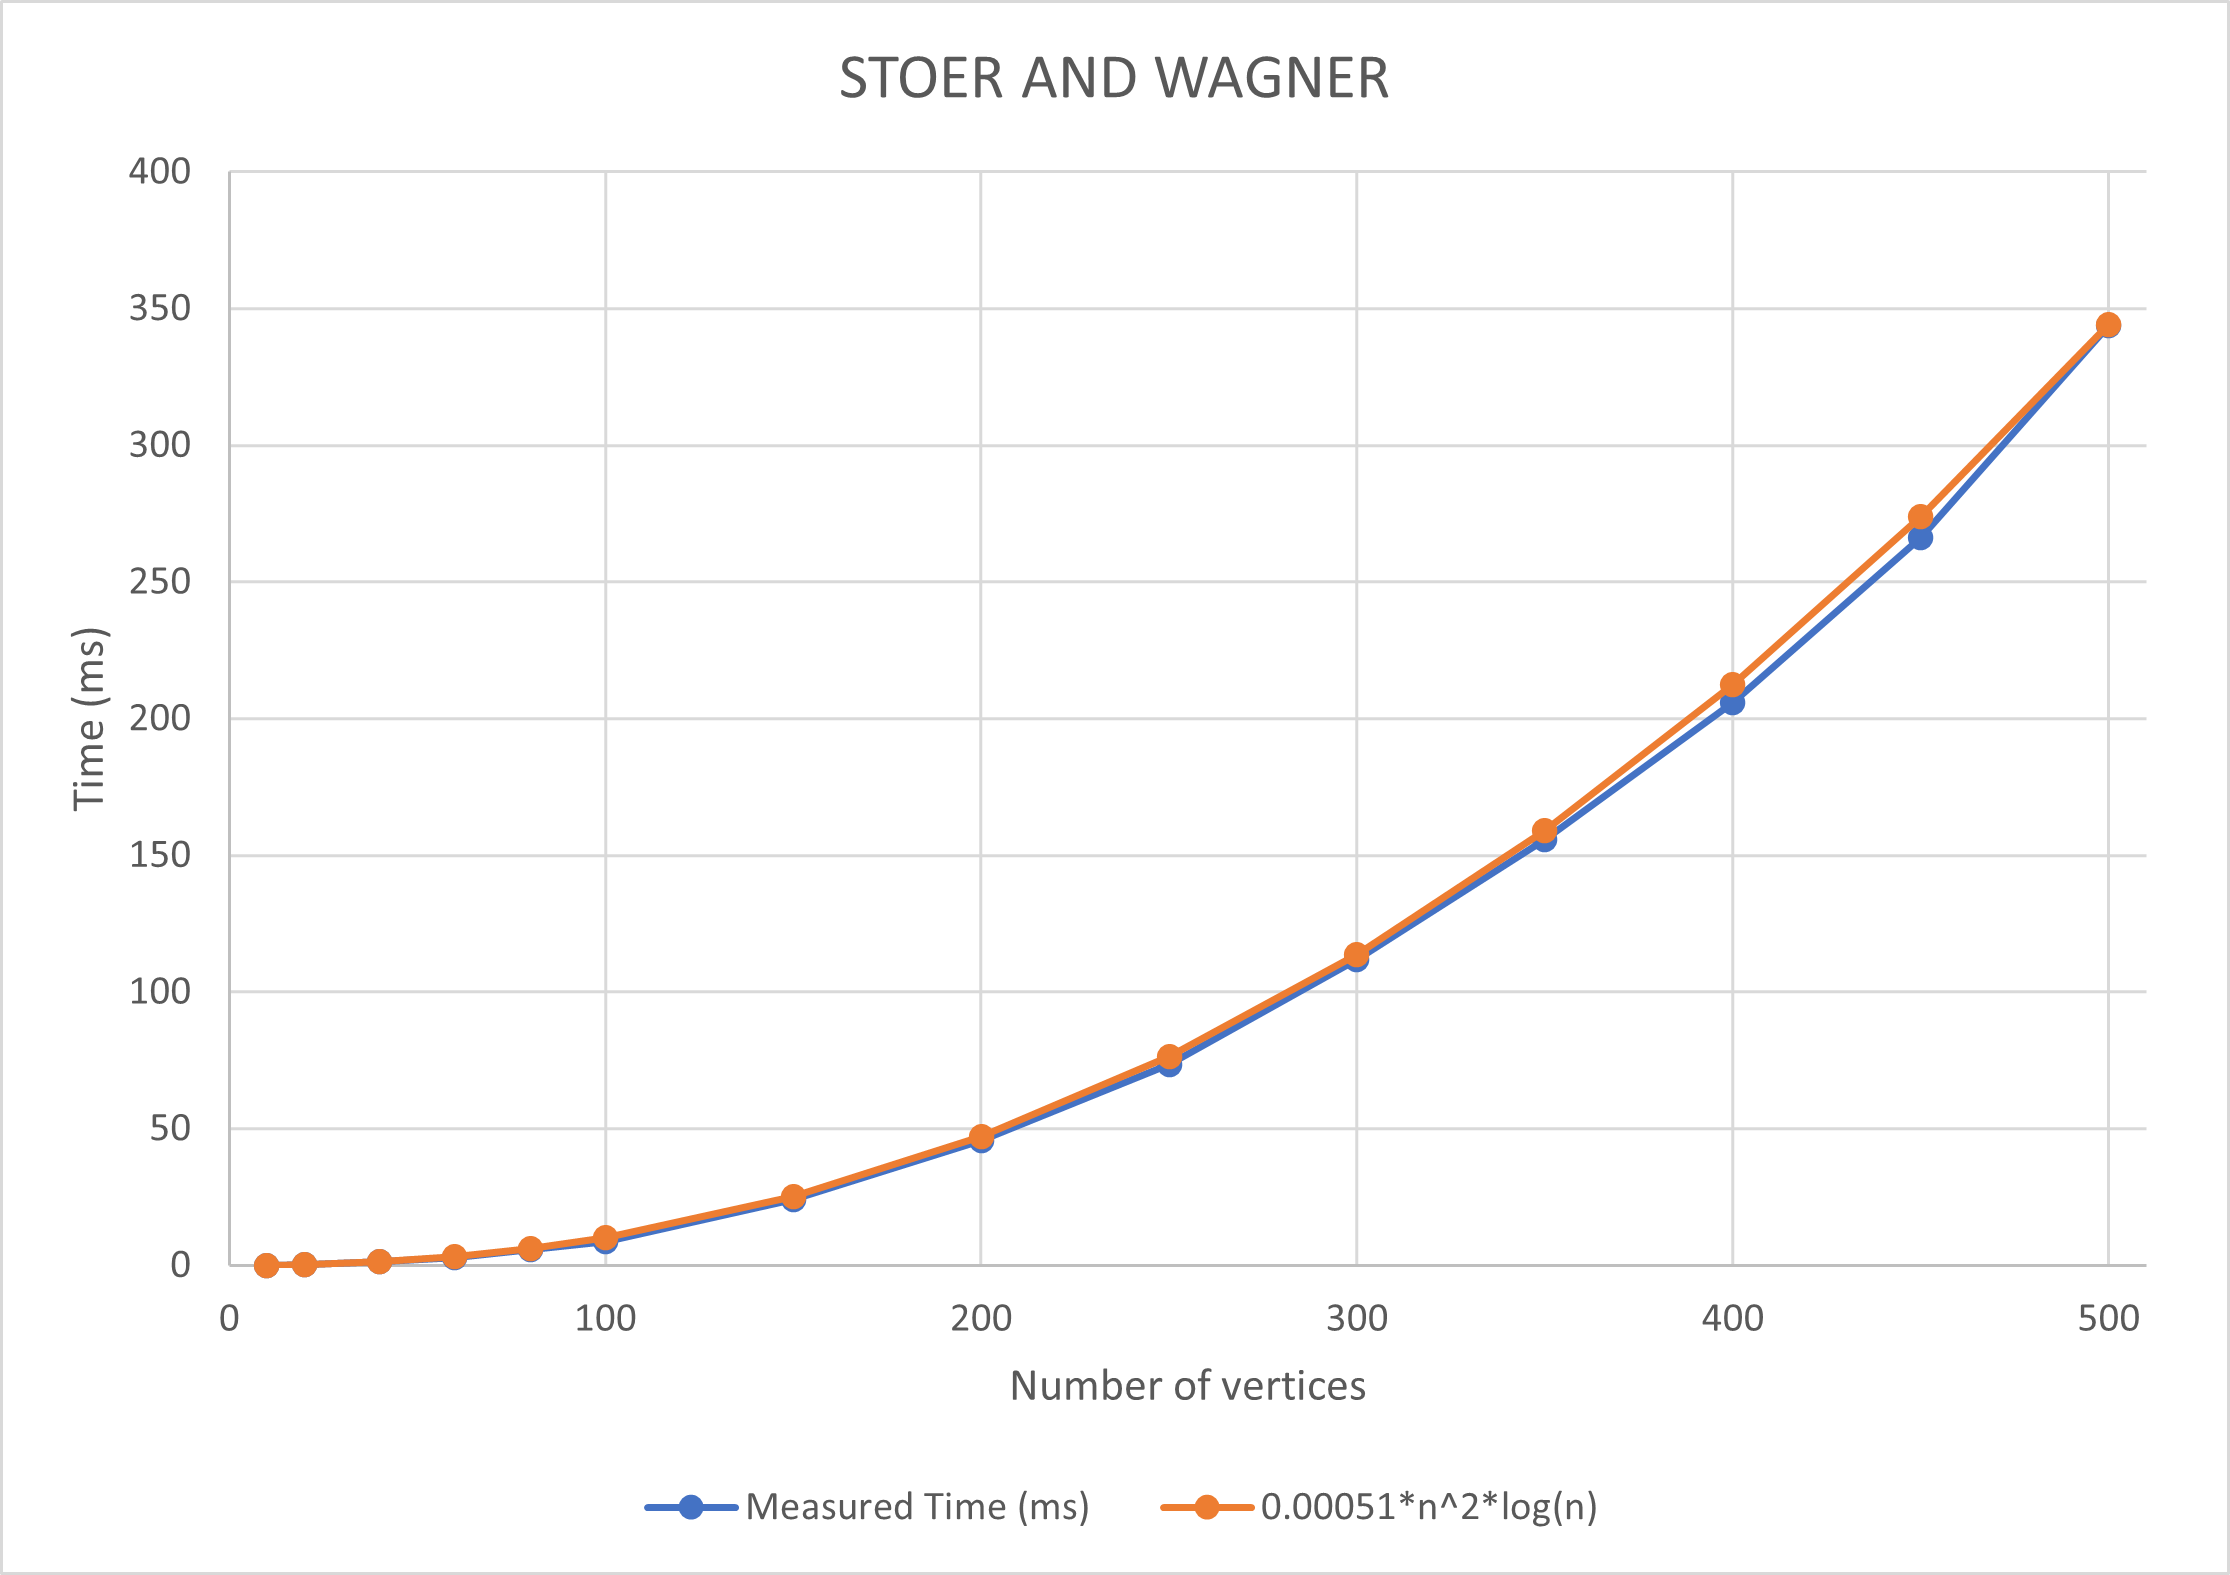
\includegraphics[width=0.77\textwidth]{./img/Stoer_Wagner}
	\caption{Complexity of Stoer-Wagner with \textit{k} repetitions for each quartet of graphs with equal number of vertices.}
	\label{fig:stoerwagner}
\end{figure}
\noindent
The chart just illustrated above (fig. \ref{fig:stoerwagner}) shows the excepted (in orange) and actual (in blue) computational complexity for Stoer-Wagner's algorithm with more computation of the algorithm.\\ \noindent
As we can see from the figure, the complexity of the algorithm that we have implemented follows almost perfectly the asymptotic one. This is due to the optimizations that we put into the code. For this reason, it was not necessary to set up a timeout to block the execution of the algorithm.\\ \noindent
As for Stoer-Wagner, also for the Karger and Stein's algorithm we have implemented the code in C\# for the execution of the algorithm on the whole provided dataset. The results are also reported in detail with the relative weights also in the appendix section (\ref{stoer}).\\ \noindent
In the figure \ref{fig:kargerstein} is reported the excepted (in orange) and actual (in blue) computational complexity for Karger and Stein's algorithm with more computation of the algorithm. It's possible to notice that the algorithm which we have implemented is slightly below the asymptotic complexity for large graphs and lightly above when the number of vertices is around 300. In general, we can see how the execution time is very similar to the time predicted by theoretical complexity.

\begin{figure}[H]
	\centering
	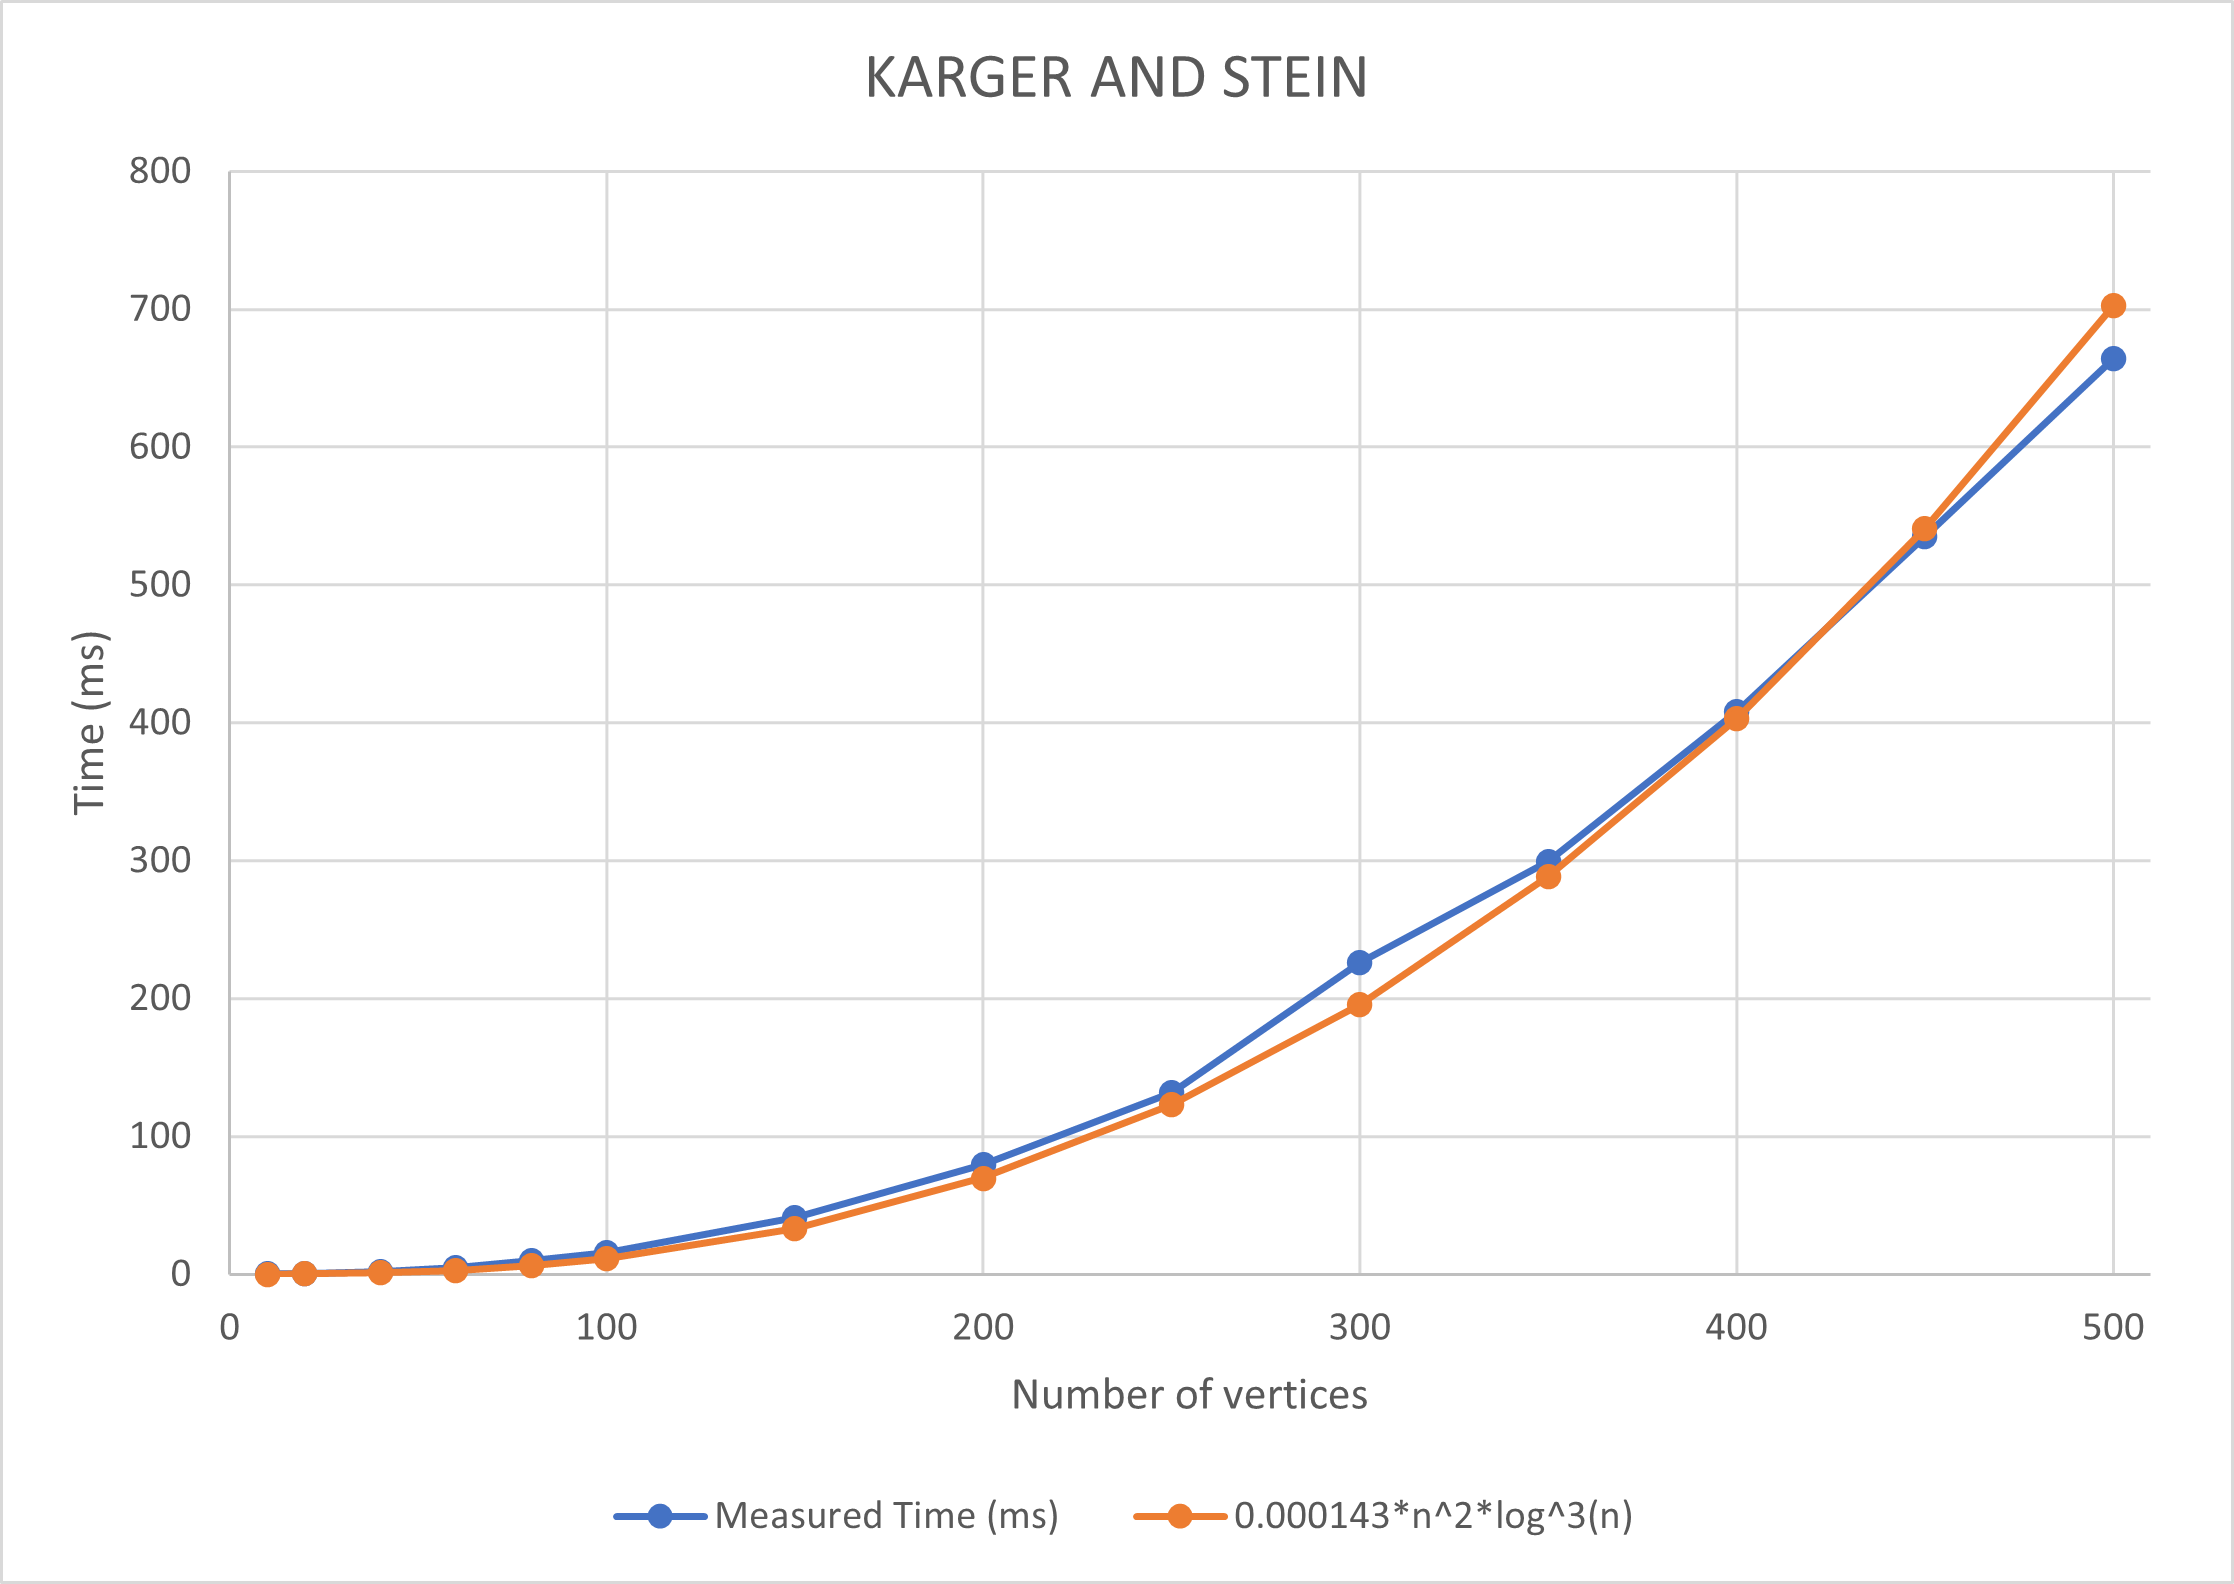
\includegraphics[width=0.77\textwidth]{./img/Karger_Stein}
	\caption{Complexity of Karger and Stein with \textit{k} repetitions for each quartet of graphs with equal number of vertices.}
	\label{fig:kargerstein}
\end{figure}
\noindent
In addition to the repetitions necessary to perform correctly the measurements, the Karger and Stein's algorithm requires that the procedure for calculating the minimum cut is repeated a sufficient number of times, such that the algorithm has a probability less than or equal to \(\frac{1}{n}\) of making mistakes. Therefore, the number of repetitions that satisfies this constraint is equal to $log{_2}^2(n)$.\\ \\ \noindent
An analysis that was carried out more for simple curiosity than for a practical reason, concerns the number of minimum iterations in which the algorithm is able to determine the min-cut. It was possible to notice that compared to the $log{_2}^2(n)$ repetitions that the algorithm needs for the high probability, the Karger and Stein's algorithm was able to determine the min-cut in a much smaller number of iterations. Below are the graphs of the analysis just described:
\begin{figure}[H]
	\centering
	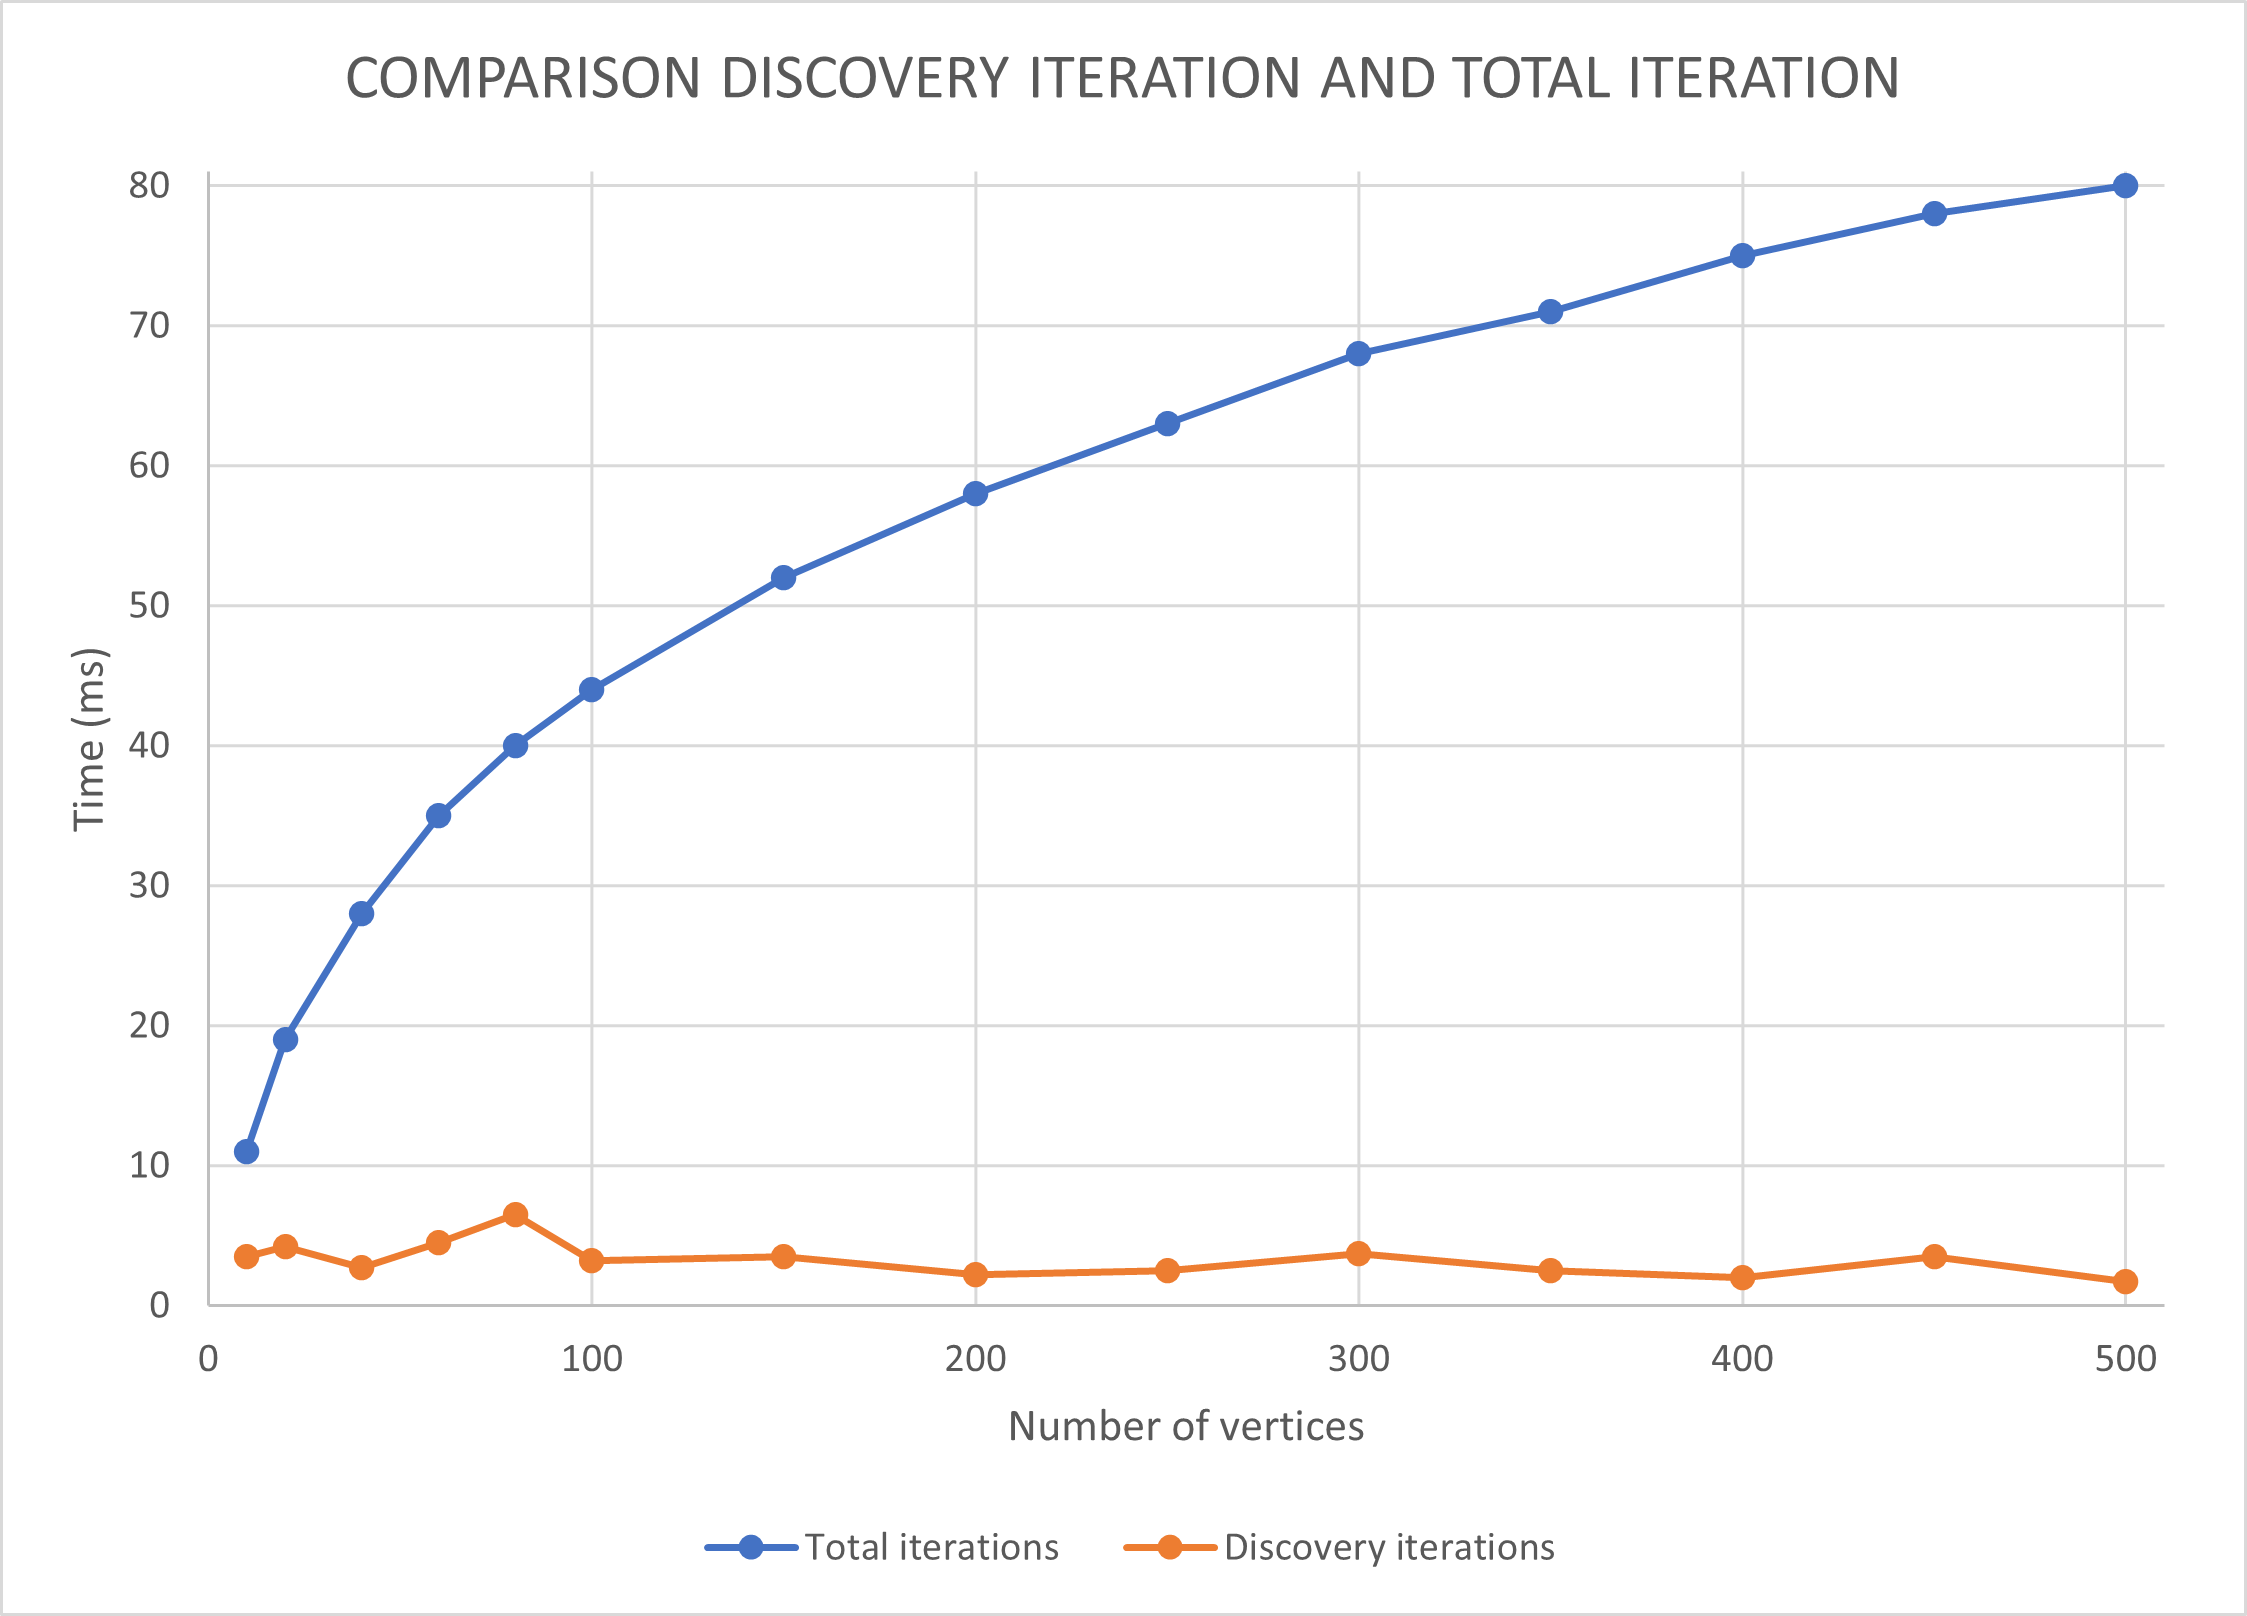
\includegraphics[width=0.77\textwidth]{./img/ComparisonTotalDiscoveryIteration}
	\caption{Comparison between the number of iterations needed to determine the min-cut and the total number of iterations.}
	\label{fig:kargerComparisonIteration}
\end{figure}
\begin{figure}[H]
	\centering
	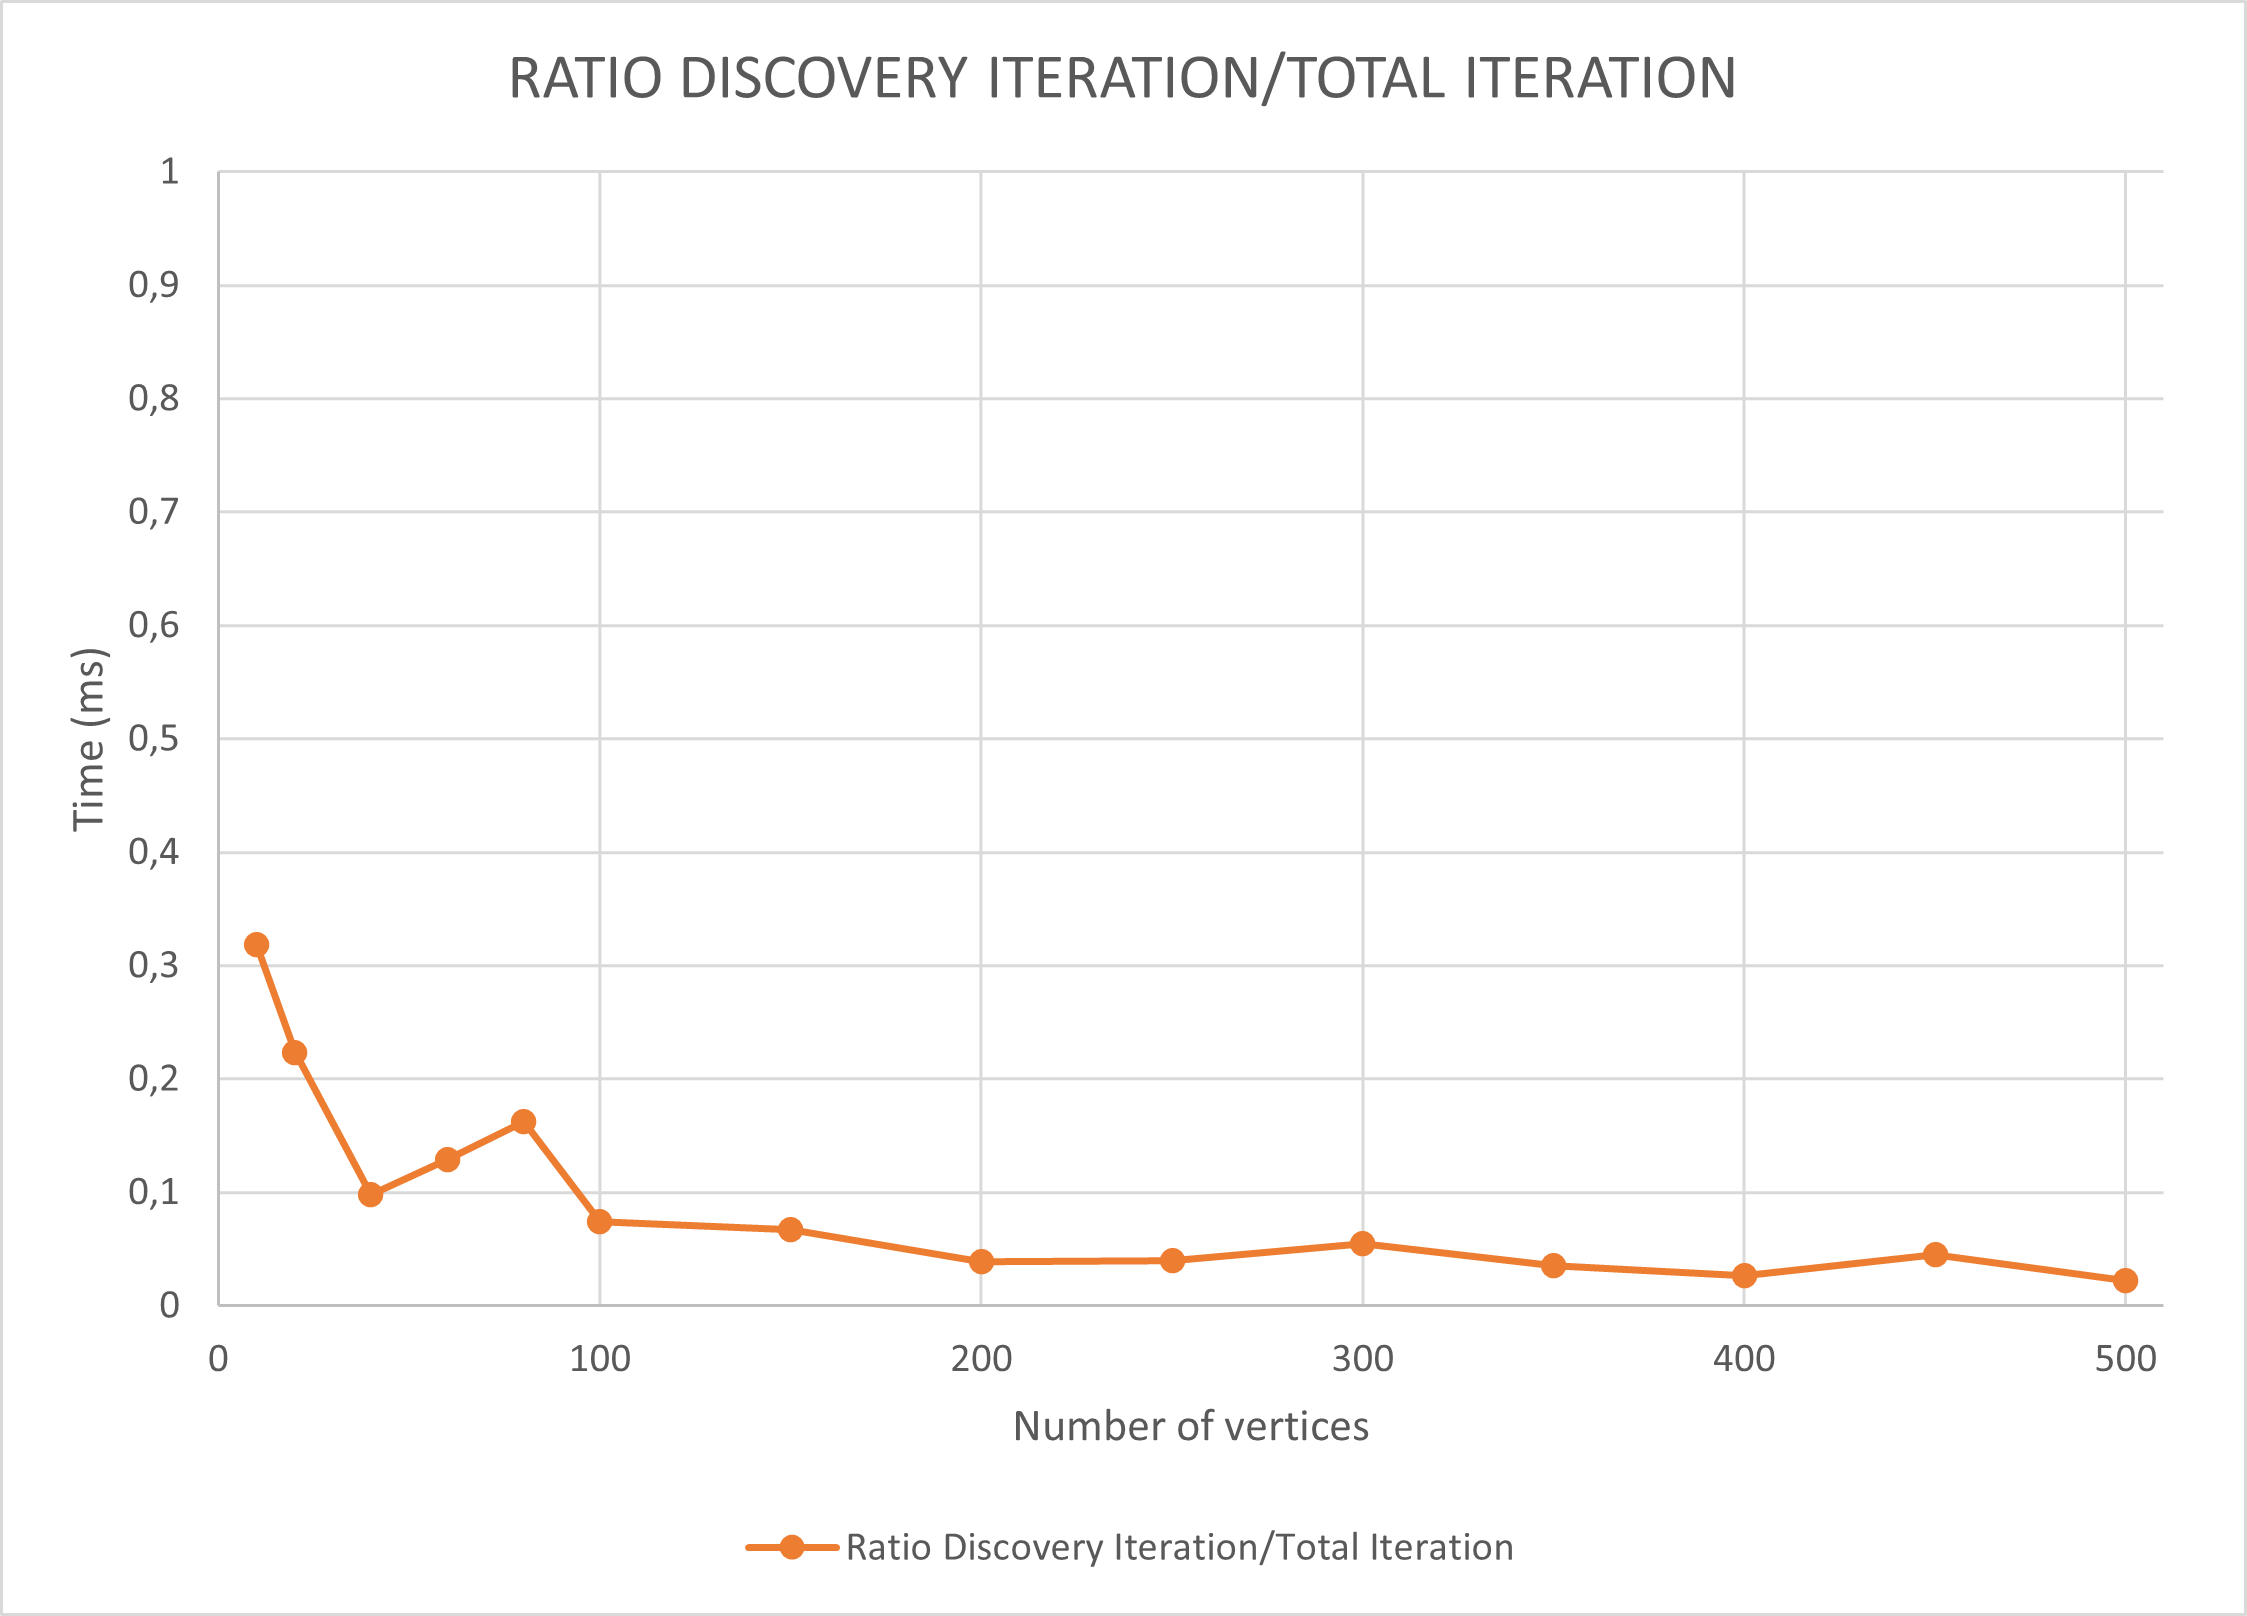
\includegraphics[width=0.77\textwidth]{./img/RatioTotalDiscoveryIteration}
	\caption{Ratio between the number of iterations needed to determine the min-cut and the total number of iterations.}
	\label{fig:kargerComparisonIteration}
\end{figure}
\noindent
\pagebreak
\subsection{Question 2}
\textit{Measure the discovery time of the Karger and Stein algorithm. The discovery time is the instant (in seconds) when the algorithm finds the minimum cost cut. Compare the discovery time with the overall execution time for each of the graphs in the dataset.} \\ \\ \noindent
\begin{figure}[H]
    \centering
		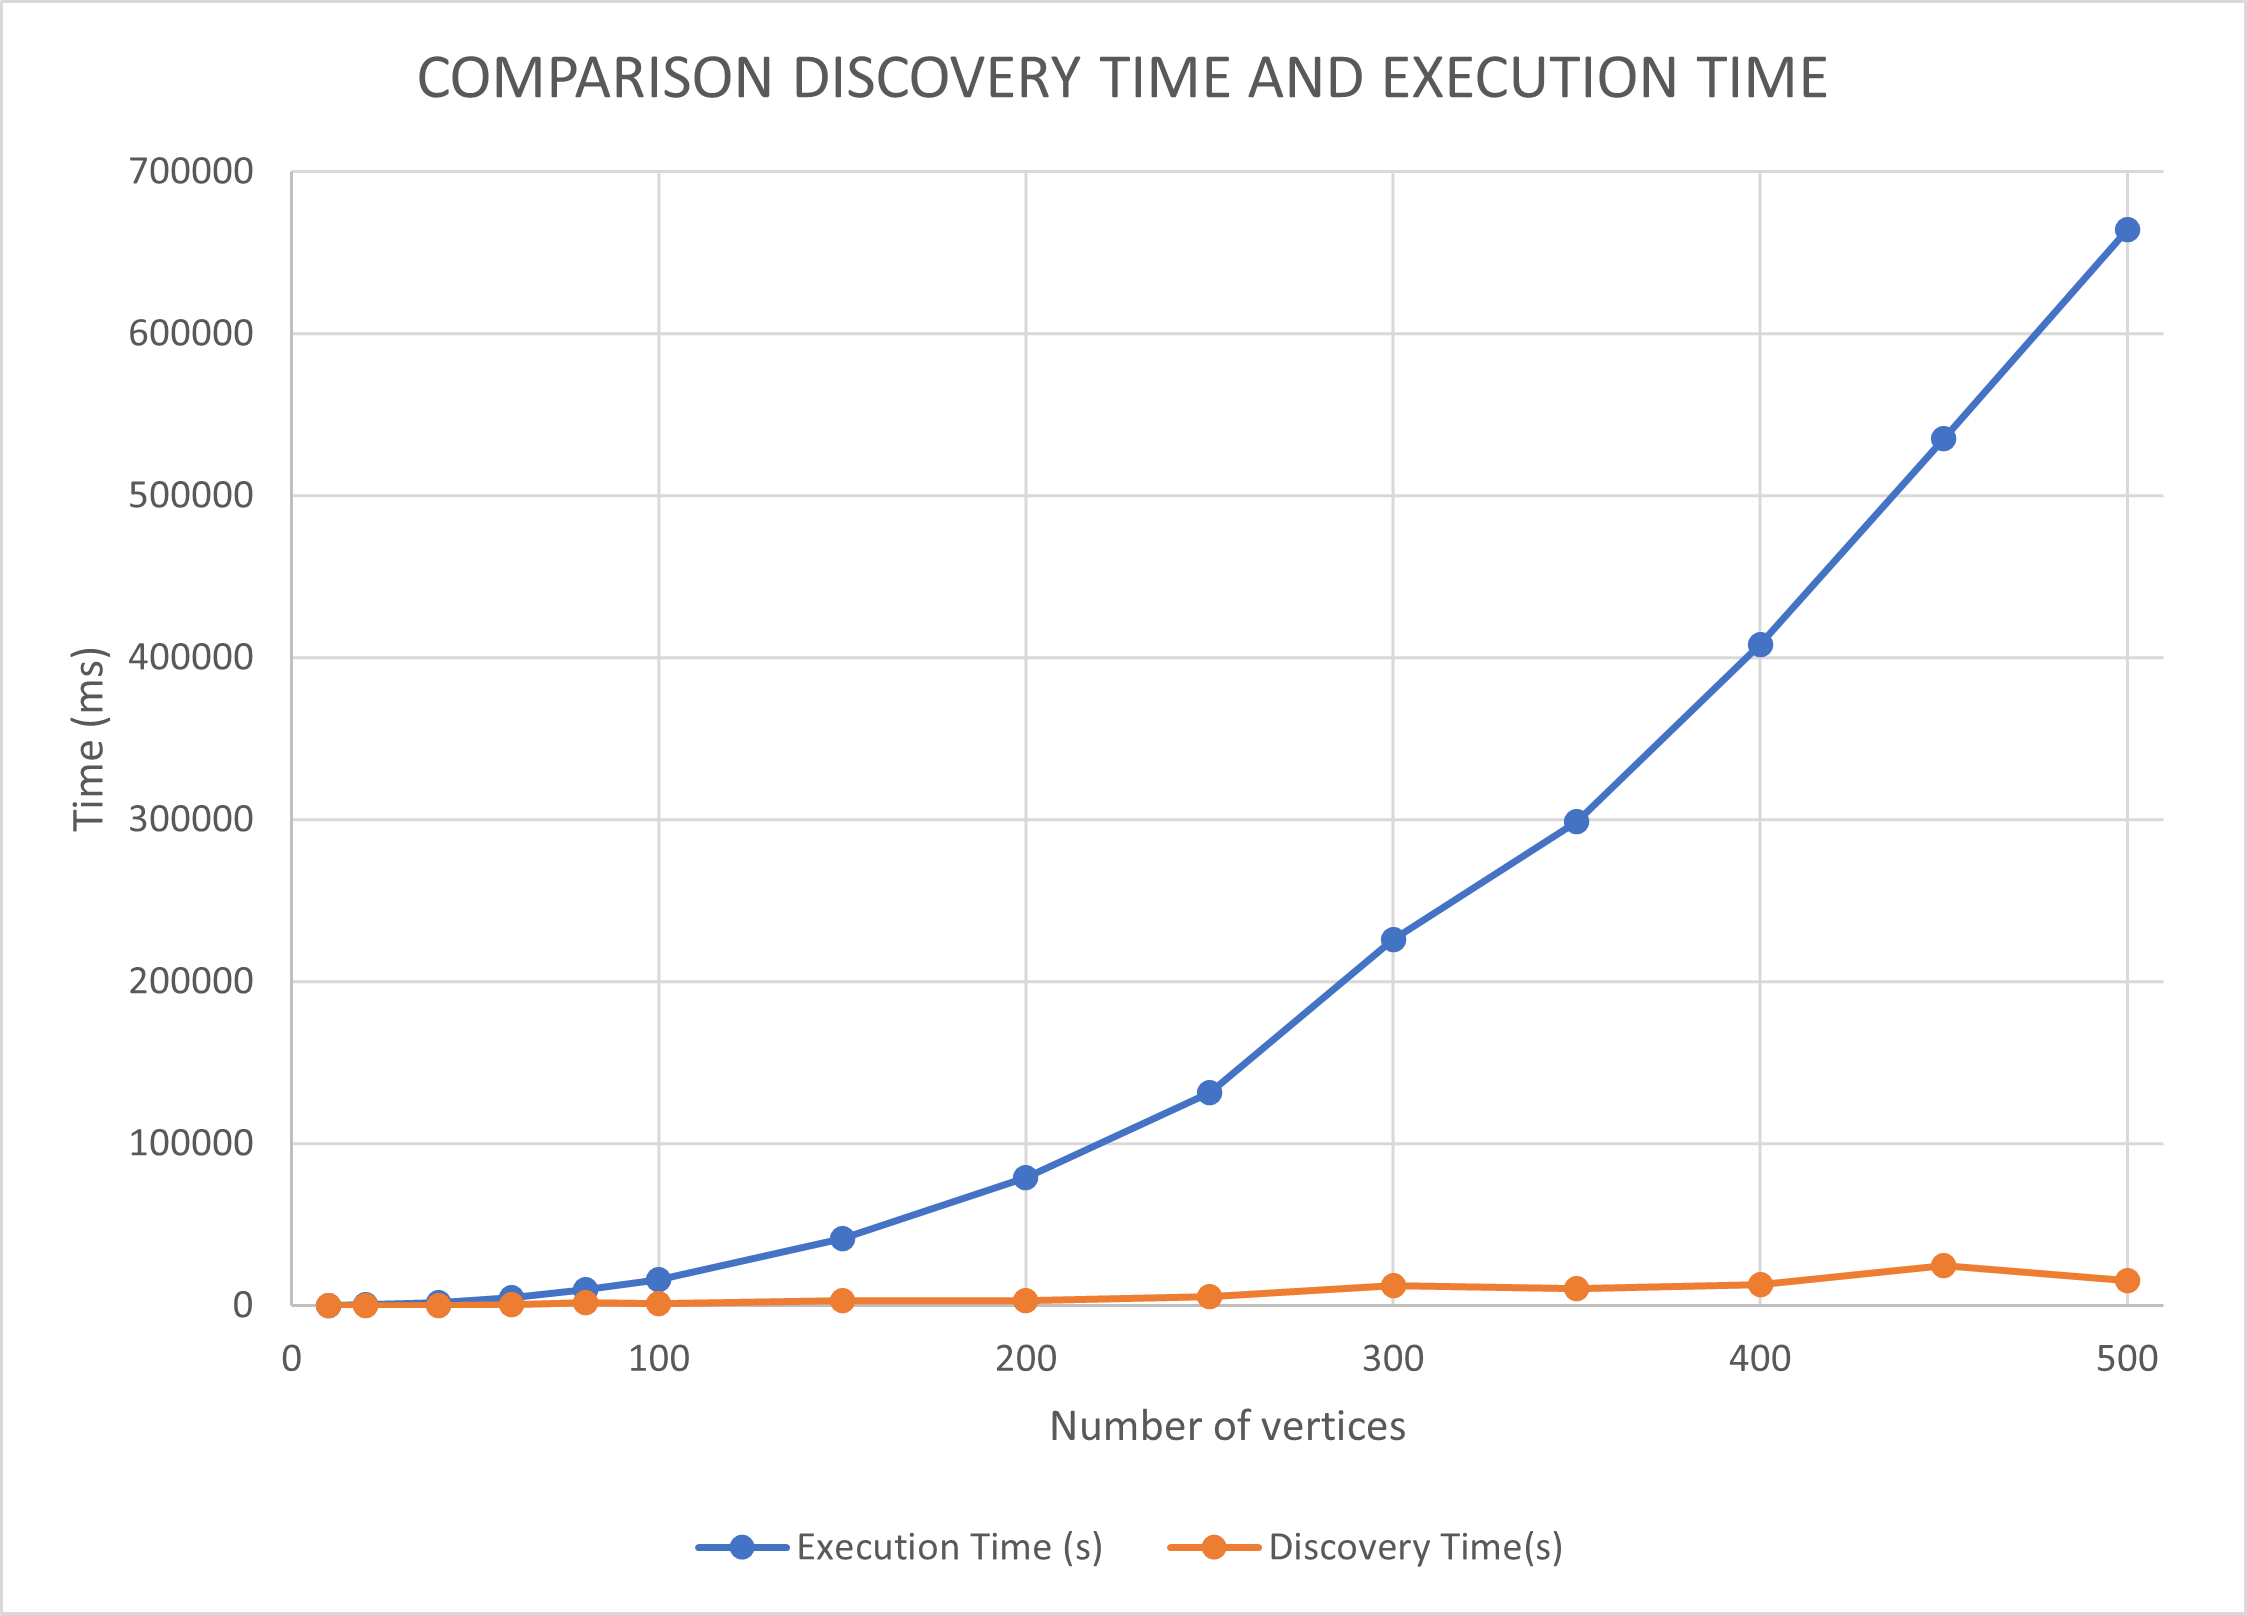
\includegraphics[width=.73\textwidth]{./img/ComparisonExecutionDiscovery.png}
		\caption{Comparison between the discovery time and the total execution time.}
		\label{fig:comparisonExecutionDiscovery}
\end{figure}
\begin{figure}[H]
    \centering
	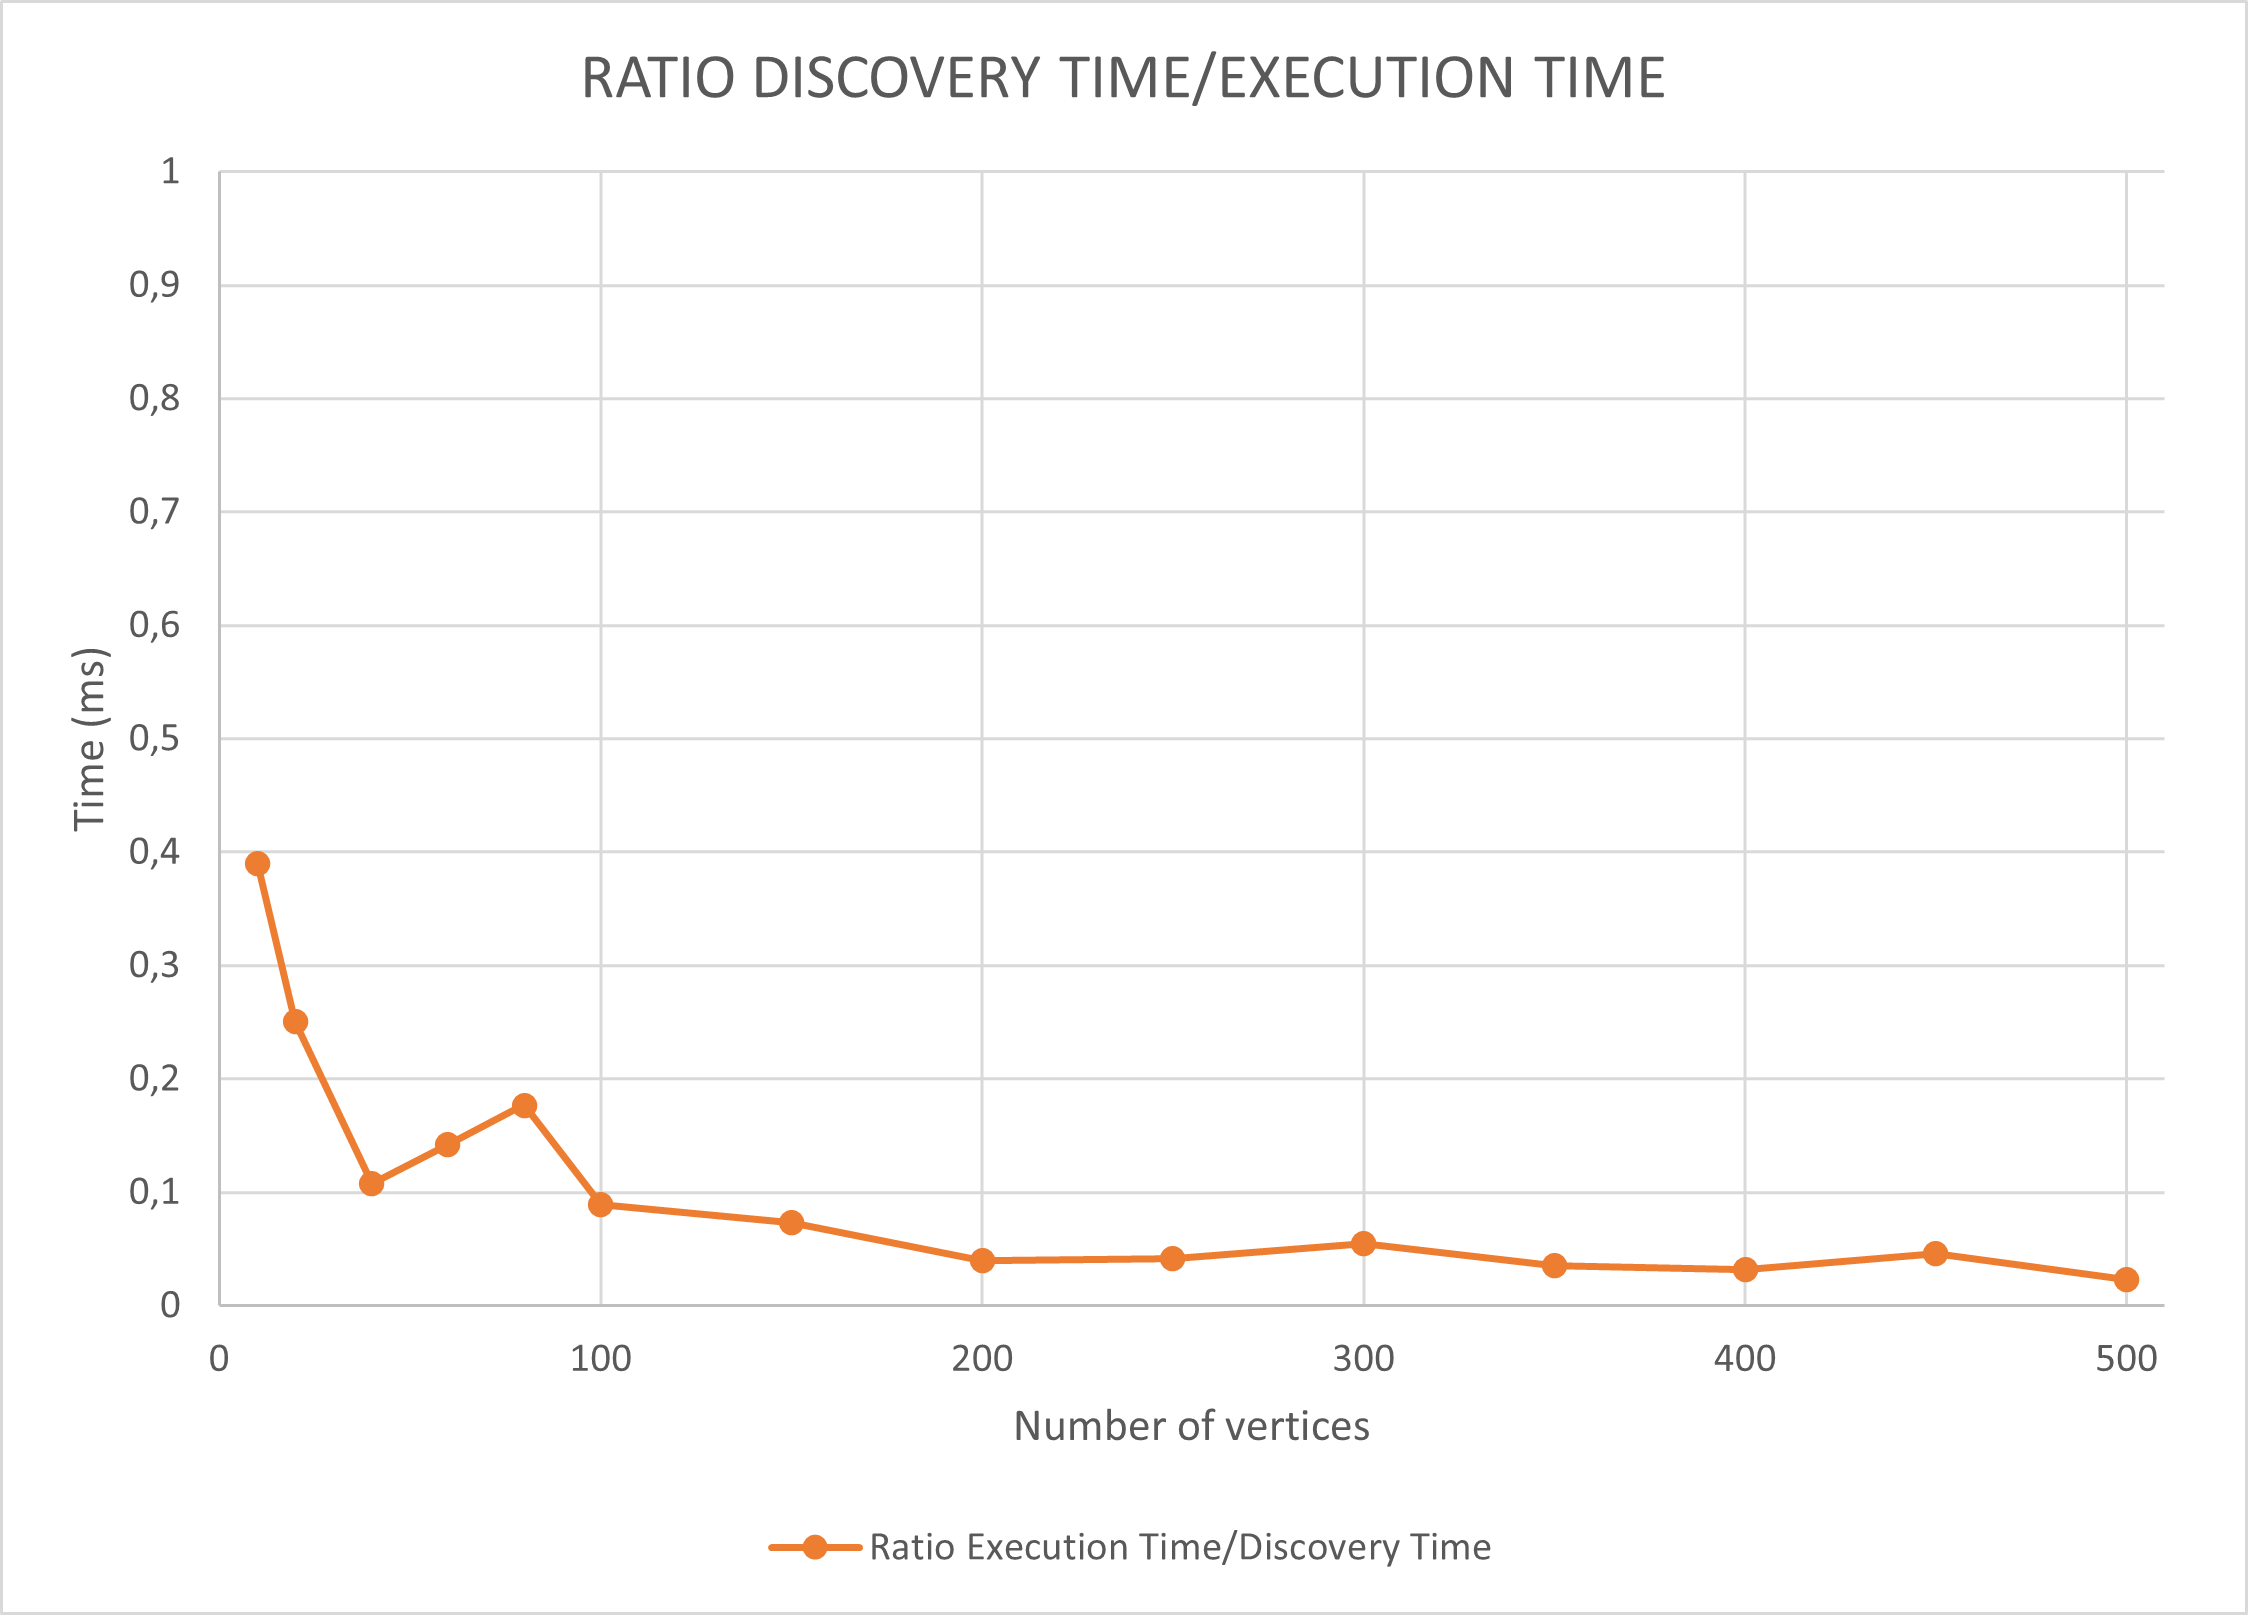
\includegraphics[width=.73\textwidth]{./img/RatioExecutionDiscovery.png}
	\caption{Ratio between the discovery time and the total execution time.}
	\label{fig:ratioExecutionDiscovery}
\end{figure}
\noindent
The values in the figure \ref{fig:ratioExecutionDiscovery} refer to the percentage of time it takes to find the minimum cut for the first time, with respect to the total execution time of the algorithm. \\ \noindent
We can see by the charts that for the smallest instances, the ratio between the discovery time and the total execution time is higher than for larger instances. Since we have no upper limit to the total execution time, having not used any type of threshold, we can see how the percentage tends to go down and we are able also to obtain more precise solution, in particular, the Karger and Stein's algorithm always returns the optimal solution.

\subsection{Question 3}
\textit{Comment on the results you have obtained: how do the algorithms behave with respect to the various instances? There is an algorithm that is always better than the other? Which algorithm is more efficient?}\\ \\
\noindent
The results obtained by the two algorithms are perfectly in line with what we expected the theoretical point of view. The trend of the various instances is in line with the asymptotic complexity, in fact as the number of nodes increases, the execution time of the algorithm we have implemented correspondingly increases.\\ \noindent
Analyzing the execution times of the two algorithms we can affirm that the Stoer-Wagner's algorithm is significantly faster than the Karger and Stein's algorithm, with a maximum time in the larger instance equal to 21 milliseconds, while the second takes more than 333 milliseconds with the repetitions with high probability. Hence Stoer-Wagner is therefore the best algorithm in relation to computational time and discovery time. Comparing it with Karger and Stein's algorithm in terms of efficiency and precision we can see that the reported results are correct. In conclusion, it can be said that the best algorithm, for how we have implemented them, is Stoer-Wagner.